% A LaTeX template for EXECUTIVE SUMMARY of the MSc Thesis submissions to 
% Politecnico di Milano (PoliMi) - School of Industrial and Information Engineering
%
% S. Bonetti, A. Gruttadauria, G. Mescolini, A. Zingaro
% e-mail: template-tesi-ingind@polimi.it
%
% Last Revision: October 2021
%
% Copyright 2021 Politecnico di Milano, Italy. NC-BY

\documentclass[11pt,a4paper,twocolumn]{article}

%------------------------------------------------------------------------------
%	REQUIRED PACKAGES AND  CONFIGURATIONS
%------------------------------------------------------------------------------
% PACKAGES FOR TITLES
\usepackage{titlesec}
\usepackage{color}

% PACKAGES FOR LANGUAGE AND FONT
\usepackage[utf8]{inputenc}
\usepackage[english]{babel}
\usepackage[T1]{fontenc} % Font encoding

% PACKAGES FOR IMAGES
\usepackage{graphicx}
\graphicspath{{Images/}} % Path for images' folder
\usepackage{eso-pic} % For the background picture on the title page
\usepackage{subfig} % Numbered and caption subfigures using \subfloat
\usepackage{caption} % Coloured captions
\usepackage{transparent}

% STANDARD MATH PACKAGES
\usepackage{amsmath}
\usepackage{amsthm}
\usepackage{bm}
\usepackage[overload]{empheq}  % For braced-style systems of equations

% PACKAGES FOR TABLES
\usepackage{tabularx}
\usepackage{longtable} % tables that can span several pages
\usepackage{colortbl}

% PACKAGES FOR ALGORITHMS (PSEUDO-CODE)
\usepackage{algorithm}
\usepackage{algorithmic}

% PACKAGES FOR REFERENCES & BIBLIOGRAPHY
\usepackage[colorlinks=true,linkcolor=black,anchorcolor=black,citecolor=black,filecolor=black,menucolor=black,runcolor=black,urlcolor=blue]{hyperref} % Adds clickable links at references
\usepackage{cleveref} % Optional: cross-references with automatic handling of "Figure", "Table", etc.
\usepackage[backend=biber, style=numeric, sorting=none, url=true]{biblatex} % Use BibLaTeX with biber backend
\addbibresource{bibliography.bib} % Path to your .bib file
\usepackage[hyphenbreaks]{breakurl} % Better handling of long URLs


% PACKAGES FOR THE APPENDIX
\usepackage{appendix}

% PACKAGES FOR ITEMIZE & ENUMERATES 
\usepackage{enumitem}

% OTHER PACKAGES
\usepackage{amsthm,thmtools,xcolor} % Coloured "Theorem"
\usepackage{comment} % Comment part of code
\usepackage{fancyhdr} % Fancy headers and footers
\usepackage{lipsum} % Insert dummy text
\usepackage{tcolorbox} % Create coloured boxes (e.g. the one for the key-words)
\usepackage{stfloats} % Correct position of the tables


%-------------------------------------------------------------------------
%	NEW COMMANDS DEFINED
%-------------------------------------------------------------------------
% EXAMPLES OF NEW COMMANDS -> here you see how to define new commands
\newcommand{\bea}{\begin{eqnarray}} % Shortcut for equation arrays
\newcommand{\eea}{\end{eqnarray}}
\newcommand{\e}[1]{\times 10^{#1}}  % Powers of 10 notation
\newcommand{\mathbbm}[1]{\text{\usefont{U}{bbm}{m}{n}#1}} % From mathbbm.sty
\newcommand{\pdev}[2]{\frac{\partial#1}{\partial#2}}
% NB: you can also override some existing commands with the keyword \renewcommand


%----------------------------------------------------------------------------
%	ADD YOUR PACKAGES (be careful of package interaction)
%----------------------------------------------------------------------------


%----------------------------------------------------------------------------
%	ADD YOUR DEFINITIONS AND COMMANDS (be careful of existing commands)
%----------------------------------------------------------------------------


% Do not change Configuration_files/config.tex file unless you really know what you are doing. 
% This file ends the configuration procedures (e.g. customizing commands, definition of new commands)
% Set the geometric layout of the document
\usepackage{geometry}
\geometry{
  top=3cm,
  left = 2.0cm,
  right = 2.0cm,
  bottom=2cm,
  headheight= 2cm,
  headsep= 0cm,
}
\raggedbottom 

\definecolor{redTn}{RGB}{177, 11, 37}

% Custom theorem environments
\declaretheoremstyle[
  headfont=\color{redTn}\normalfont\bfseries,
  bodyfont=\color{black}\normalfont\itshape,
]{colored}

\captionsetup[figure]{labelfont={color=redTn}} % Set colour of the captions
\captionsetup[table]{labelfont={color=redTn}} % Set colour of the captions
\captionsetup[algorithm]{labelfont={color=redTn}} % Set colour of the captions

\theoremstyle{colored}
\newtheorem{theorem}{Theorem}[section]
\newtheorem{proposition}{Proposition}[section]

% Enhances the features of the standard "table" and "tabular" environments.
\newcommand\T{\rule{0pt}{2.6ex}}
\newcommand\B{\rule[-1.2ex]{0pt}{0pt}}

% Algorithm description
\newcounter{algsubstate}
\renewcommand{\thealgsubstate}{\alph{algsubstate}}
\newenvironment{algsubstates}{
    \setcounter{algsubstate}{0}%
    \renewcommand{\STATE}{%
    \stepcounter{algsubstate}%
    \Statex {\small\thealgsubstate:}\space}
    }{}
    
% Custom theorem environment
\newcolumntype{L}[1]{>{\raggedright\let\newline\\\arraybackslash\hspace{0pt}}m{#1}}
\newcolumntype{C}[1]{>{\centering\let\newline\\\arraybackslash\hspace{0pt}}m{#1}}
\newcolumntype{R}[1]{>{\raggedleft\let\newline\\\arraybackslash\hspace{0pt}}m{#1}}

% Custom itemize environment
\setlist[itemize,1]{label=$\bullet$}
\setlist[itemize,2]{label=$\circ$}
\setlist[itemize,3]{label=$-$}
\setlist{nosep}

% Set separation of columns 
\setlength{\columnsep}{30pt}

% Set indentation
\setlength\parindent{0pt}

% Custom title commands
\titleformat{\section}
{\color{redTn}\normalfont\Large\bfseries}
{\color{redTn}\thesection.}{1em}{}
\titlespacing*{\section}
{0pt}{2ex}{1ex}

\titleformat{\subsection}
{\color{redTn}\normalfont\large\bfseries}
{\color{redTn}\thesubsection.}{1em}{}
\titlespacing*{\subsection}
{0pt}{2ex}{1ex}

% Custom headers and footers
\pagestyle{fancy}
\fancyhf{}
      
\fancyfoot{}
\fancyfoot[C]{\thepage} % page
\renewcommand{\headrulewidth}{0mm} % headrule width
\renewcommand{\footrulewidth}{0mm} % footrule width

\makeatletter
\patchcmd{\headrule}{\hrule}{\color{black}\hrule}{}{} % headrule
\patchcmd{\footrule}{\hrule}{\color{black}\hrule}{}{} % footrule
\makeatother

% -> Create the header
\chead[C]{
\centering
\begin{tcolorbox}[arc=0pt, boxrule=0pt, colback=redTn!60, width=\textwidth, colupper=white]
    \textbf{ASA - Deliveroo Report} \hfill \textbf{\author}  
\end{tcolorbox}
}


\usepackage{listings}
\lstset{
  basicstyle=\ttfamily\small,
  keywordstyle=\bfseries,
  commentstyle=\itshape,
  breaklines=true
}



\definecolor{lightgray}{rgb}{.9,.9,.9}
\definecolor{darkgray}{rgb}{.4,.4,.4}
\definecolor{purple}{rgb}{0.65, 0.12, 0.82}

\lstdefinelanguage{JavaScript}{
  keywords={typeof, new, true, false, catch, function, return, null, catch, switch, var, if, in, while, do, else, case, break},
  keywordstyle=\color{blue}\bfseries,
  ndkeywords={class, export, boolean, throw, implements, import, this},
  ndkeywordstyle=\color{darkgray}\bfseries,
  identifierstyle=\color{black},
  sensitive=false,
  comment=[l]{//},
  morecomment=[s]{/*}{*/},
  commentstyle=\color{olive}\ttfamily,
  stringstyle=\color{red}\ttfamily,
  morestring=[b]',
  morestring=[b]"
}

\lstset{
   language=JavaScript,
   backgroundcolor=\color{lightgray},
   extendedchars=true,
   basicstyle=\footnotesize\ttfamily,
   showstringspaces=false,
   showspaces=false,
   numbers=none,
   numberstyle=\footnotesize,
   numbersep=9pt,
   tabsize=2,
   breaklines=true,
   showtabs=false,
   captionpos=b
}



% Insert here the info that will be displayed into your Title page 
% -> title of your work
\renewcommand{\title}{Autonomous Software Agents}
% -> author name and surname
\renewcommand{\author}{Matteo Bando, Jonathan Fin}
\newcommand{\authorinfo}{259068, matteo.bando@studenti.unitn.it; 256178, jonathan.fin@studenti.unitn.it}
% -> MSc course
\newcommand{\course}{Artificial Intelligence Systems}
% -> advisor name and surname
% \newcommand{\advisor}{Prof. Carlo Casonato, Prof. Simone Penasa}
% IF AND ONLY IF you need to modify the co-supervisors you also have to modify the file Configuration_files/title_page.tex (ONLY where it is marked)
% \newcommand{\firstcoadvisor}{Name Surname} % insert if any otherwise comment
%\newcommand{\secondcoadvisor}{Name Surname} % insert if any otherwise comment
% -> academic year
\newcommand{\YEAR}{2024-2025}

%-------------------------------------------------------------------------
%	BEGIN OF YOUR DOCUMENT
%-------------------------------------------------------------------------
\begin{document}

%-----------------------------------------------------------------------------
% TITLE PAGE
%-----------------------------------------------------------------------------
% Do not change Configuration_files/TitlePage.tex (Modify it IF AND ONLY IF you need to add or delete the Co-advisors)
% This file creates the Title Page of the document
% DO NOT REMOVE SPACES BETWEEN LINES!

\twocolumn[{\begin{@twocolumnfalse}

\AddToShipoutPicture*{\BackgroundPic}

\begin{center}
\hspace{-0.6cm}
\includegraphics[width=0.6\textwidth]{unitn-logo.png}
\end{center}

% \vspace{-1mm}
% \fontsize{0.3cm}{0.5cm}\selectfont \bfseries \textsc{\color{redTn} Report}\\

\vspace{-0.2cm}
\Large{\textbf{\color{redTn}{\title}}}\\

\vspace{-0.2cm}
\fontsize{0.3cm}{0.5cm}\selectfont \bfseries \textsc{\color{redTn} Master's Degree in \course}\\

\vspace{-0.2cm}
\fontsize{0.3cm}{0.5cm} \selectfont \bfseries Authors: \textsc{\textbf{\author}}\\

\vspace{-0.5cm}
\fontsize{0.3cm}{0.5cm} \selectfont \bfseries IDs and e-mails:
\authorinfo \\

% \vspace{-0.4cm}
% \fontsize{0.3cm}{0.5cm}\selectfont \bfseries Professors: \textsc{\textbf{\advisor}}\\

% if only ONE co-advisor is present:
% \vspace{-0.4cm}
% \fontsize{0.3cm}{0.5cm}\selectfont \bfseries Co-advisor: \textsc{\textbf{\firstcoadvisor}}\\
% if more than one co-advisors are present:
%\vspace{-0.4cm}
%\fontsize{0.3cm}{0.5cm}\selectfont \bfseries Co-advisors: \textsc{\textbf{\firstcoadvisor}}\textsc{\textbf{\secondcoadvisor}}\\

\vspace{-0.4cm}
\fontsize{0.3cm}{0.5cm}\selectfont \bfseries Academic year: \textsc{\textbf{\YEAR}}

\small \normalfont

\vspace{11pt}

\centerline{\rule{1.0\textwidth}{0.4pt}}

\vspace{15pt}
\end{@twocolumnfalse}}]

\thispagestyle{plain} % In order to not show the header in the first page

\tableofcontents

\section{Introduction}
Deliveroo.js is a two-dimensional, grid-based parcel‐delivery game designed to offer an interactive environment where autonomous agents compete to achieve the highest score while dynamically refining their planning strategies.

\bigskip

\textbf{Map and Environment:} at the start of each match, agents are placed on a map represented by a grid: each cell is either walkable or blocked. Walkable cells may also serve as delivery zones or parcel spawning sites. On a parcel-spawning cell, packages appear at random intervals, each carrying a point value that, depending on the game’s configuration, may decay over time.

\bigskip

\textbf{Parcel Handling:} to pick up a parcel, an agent must move onto its cell and execute a pick-up action; to deliver it, the agent transports it to a delivery zone and performs a drop-off. Agents can carry an unlimited number of parcels, but they only earn the points corresponding to each parcel's value at the moment of delivery, and any parcel whose timer reaches zero disappears immediately.

\bigskip

\textbf{Game Modes:} the game can be played in free-for-all mode, where every agent competes individually, or in team mode, where teams of agents collaborate. The objective in all modes is to accumulate the highest total score on the map.

\bigskip

\textbf{Match Configuration:} at the beginning of every round, all clients receive a configuration file that defines the map matrix and sets all relevant parameters, such as the observation distance or the server clock, for that specific match.


\section{Single Agent}
\subsection{Initial configuration}

When a single agent is launched, it undergoes the following initialization steps to prepare for interaction with the Deliveroo simulation server:

\begin{enumerate}
  \item \textbf{Client setup:} we instantiate \texttt{DeliverooClient}, a thin wrapper around \texttt{DeliverooApi} that centralizes connection parameters (host URL, master/slave tokens) and decouples the code from the external library. Upon construction, it registers callback hooks for all incoming events:
    \begin{itemize}
      \item \texttt{onYou} (agent identity and initial position)  
      \item \texttt{onTile} / \texttt{onMap} (map tiles and full map load)  
      \item \texttt{onConfig} (server configuration parameters)  
      \item \texttt{onParcelsSensing} (visible parcels)  
      \item \texttt{onAgentsSensing} (visible other agents)  
    \end{itemize}

  \item \textbf{Model instantiation:} the agent’s internal knowledge is organized into five core stores:
    \begin{itemize}
      \item \texttt{Me} holds the agent’s identifier, current coordinates, and status.  
      \item \texttt{ParcelsStore} tracks known parcels (pick-up/drop-off points) on the map.  
      \item \texttt{MapStore} maintains the grid layout, tile types, computed distance matrix, and sparsity metrics.  
      \item \texttt{AgentStore} records sensed positions and timestamps of other agents.  
      \item \texttt{ServerConfig} caches global simulation parameters (clock interval, map dimensions, sensing radius, carrying capacity).
    \end{itemize}

  \item \textbf{Agent injection:} we create an \texttt{Agent} instance and wire it to the client and all five stores. Its constructor signature is:
    \begin{verbatim}
new Agent(client,
          me,
          parcels,
          mapStore,
          agentStore,
          serverConfig)
\end{verbatim}
    This binds the agent’s reasoning cycle (belief update, desire generation, intention filtering, action execution) to the shared models.

  \item \textbf{Event-driven population:} as data arrives from the server, the corresponding stores are updated:
    \begin{itemize}
      \item \texttt{onYou} sets the agent’s unique ID and coordinates.  
      \item \texttt{onConfig} populates \texttt{ServerConfig} with the parameters.  
      \item \texttt{onMap} and \texttt{onTile} build the terrain graph in \texttt{MapStore} and trigger distance/sparsity pre-computations.  
      \item \texttt{onParcelsSensing} and \texttt{onAgentsSensing} refresh dynamic information about parcels and other agents.
    \end{itemize}

  \item \textbf{Readiness check:} before entering its main loop, the agent ensures that:
    \begin{itemize}
      \item Its own \texttt{ID} has been received.  
      \item The map has been fully loaded (\texttt{mapStore.mapSize > 0}).  
      \item It is not currently executing a movement command (\texttt{!agent.isMoving}).
    \end{itemize}
    Only when all conditions are satisfied does the agent proceed to its continuous “perceive–deliberate–act” cycle.
\end{enumerate}


This systematic initialization ensures that, at time zero, the agent has a consistent view of both the static environment (map topology, server rules) and the dynamic elements (parcel requests, other agents), enabling robust decision‐making from the very first simulation tick.

\subsubsection*{Map}
% Mappa presa dal onMap e calcoliamo le distanze con Floyd-Warshall
The game map is obtained mainly from the \texttt{onMap} event and sometimes from the \texttt{onTile} one, if there happens to be a change in the environment.
After all the map is loaded into the memory, the Floyd-Warshall algorithm is performed: the agent now has a distance matrix available, which contains in each cell $i, j$ the distance (in tiles) from $i$ to $j$.
With this method, the agent has a very good heuristic for future calculations, often regarding the score.


\subsubsection*{Connection config}
The connection parameters for the Deliveroo server (host URL and authentication tokens) are loaded from a \texttt{.env} file by the \texttt{Config.js} module at startup:

\begin{itemize}[nosep]
  \item \texttt{Config.js} imports \texttt{dotenv}.
  \item If no \texttt{.env} file is found, an error is printed and the application continues without valid credentials.
  \item When one is loaded, \texttt{process.env} provides three properties:
    \begin{verbatim}
const CONFIG = {
 host:       process.env.HOST,
 token:      process.env.TOKEN,
 tokenSlave: process.env.TOKEN_SLAVE
};
    \end{verbatim}
  \item The \texttt{CONFIG} object is then exported and consumed by the client, which opens the WebSocket to \texttt{host} using \texttt{token} (master) or \texttt{tokenSlave} (slave).
\end{itemize}

\noindent Example of a \texttt{.env} file:
\begin{verbatim}
HOST=`YOUR_URL_HERE'
TOKEN=`YOUR_TOKEN_HERE'
TOKEN_SLAVE=`YOUR_TOKEN_HERE'
\end{verbatim}

\subsection*{Launch Command}
Once you have configured the \texttt{.env} file , start the script by running:
\begin{verbatim}
npm run start-single
\end{verbatim}



\subsection{BDI}
\subsubsection*{Parcels sensing}
% Spiegare come gestiamo le parcel viste
The agent has a limited vision, so we can sense parcels (and later agents) only up to a certain distance, based on the game configuration.

Sensed parcels are added to the memory and if they exist, they are updated. They are identified by a unique \texttt{id}, given by the server, and other standard attributes are its coordinates, if it is carried by someone and its reward.
When the object is generated, another attribute is added, which is the distance from the nearest base, necessary for a precise theorical score calculation.

\subsubsection*{Parcels revision}
% Spiegare come gestiamo le parcel che non vediamo (facciamo scendere il punteggio)
Parcels also have an attribute for storing the timestamp at which the agent last saw them. This is used in the \textit{belief revision} to calculate an existence probability, based on the time passed and the number of agents present in the map: the higher the number of agents, the lower the probability of the parcel still being on the map, not picked up by someone.
The score of the parcels are also calculated if the agent does not sense them anymore, subtracting a value based on the decaying factor from the server configuration.

\subsubsection*{Agent sensing}
% Gestione degli altri agenti
Opponent agents are handled in the same way as parcels, being added to memory or updated when sensed. They also have an attribute that represents the direction they are moving in.

\subsubsection*{Desires and Intentions}
% Spiegare come generiamo i desires, con gli score e come vengono calcolati.
% Le intentions sono i desires sortati per score decrescente
\textit{Desire generation} is one of the core parts of the agent.

It is represented as an array of desires (or possible intentions).
Three main desires exists, which consist in the following:
\begin{itemize}
    \item \textbf{Pickup:} for every parcel in the memory a score is calculated, taking into consideration the distance to reach that parcel and the distance to reach the nearest base from that parcel.
    The score calculation is shown in equation \ref{eq:score}, with $a$ being the agent, $p$ the parcel, $b$ the nearest base with respect to $p$, and $penalty$ the decaying factor of the parcels score (e.g. 1 point each second).
    A visual representation is also available in figure \ref{fig:pickup}, where the decay in score for each parcel is considered to be 1 point for each move of the agent. 
    
    \item \textbf{Deposit:} if the agent is carrying at least one parcel, a desire to go deposit the carried parcels is added to the list with its score, calculated similar to the pickup one.
    
    \item \textbf{Explore:} the agent always has a desire to explore but its score is very low. This ensures that the explore action is executed only if there's not other possibility.
\end{itemize}

\begin{equation}    \label{eq:score}
\begin{split}    
    score = (a.carried\_score + p.reward) \\ - ((distance(a, p) + distance(p, b)) \\ * (a.carried\_amount + 1) * penalty)
\end{split}
\end{equation}

\begin{figure}
    \centering
    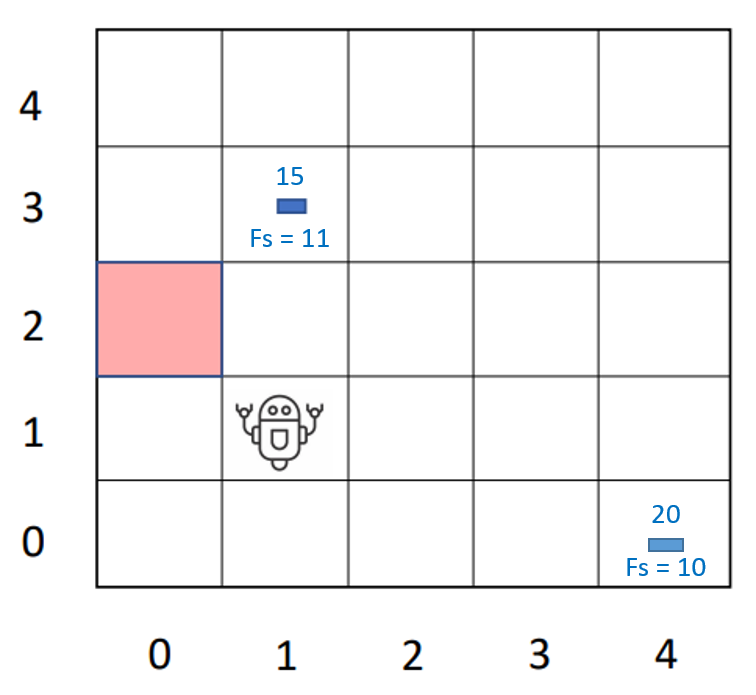
\includegraphics[width=0.9\linewidth]{Images/strategy.png}
    \caption{Pickup strategy}
    \captionsetup{font=footnotesize}
    \caption*{The number on top of the parcels is the current score, while the $Fs$ value is the final score. The red tile is the base. The agent will pickup the nearest parcel, even though the other one has a higher score currently}
    \label{fig:pickup}
\end{figure}

The desires list is then sorted by score, and the one with the highest score becomes the current intention.

% Parlare della possibile riconsiderazione delle parcel se vediamo altri agenti vicini
All the intentions are immediately transformed into an action, preceded by a planning phase, except for the \texttt{pickup} intention.
If the agent detects that another agent is going to get to the parcels faster them itself, it discard that intention and picks the second best one, perfoming again the checks if it is another \texttt{pickup} intention.
The pseudo-code for the \textit{agent-check} is the following:

\begin{lstlisting}[caption={Opponent agents checks}]
if a senses another agent:
    if agent is closer than a:
        if agent is 1 tile away from parcel OR going towards the parcel:
            discard parcel and pick next intention
\end{lstlisting}



If the opponent agent is next to the parcel it is assumed to pick up that parcel. The \textit{"going towards the parcel"} part is computed by analyzing the direction in which the agent is going, with respect to the parcel location.



\subsection{Actions}

The agent moves continuously in the map. Each path is calculated before acting, in a \textit{planning-like} phase, with the $A^*$ algorithm. 

\subsubsection*{Pickup}
% Spiegare cosa fa l'agent quando vuole fare pickup
The agent performs the \texttt{pickup} action by going to the location of the parcel and then picking it up.

\subsubsection*{Deposit}
% Spiegare cosa fa l'agent quando vuole fare deposit
The deposit intention is fulfilled by going to the nearest available home and deposit all of the carried parcels, and removing them from the memory.

\subsubsection*{Explore}
% Parlare di come avviene l'explore e il camping
If the selected intention is to \texttt{explore}, then the agent selected a reachable random spawn tile and goes to that location. If the map is \textit{sparse}, it stays on the same cell from a small period of time, waiting for a parcel to spawn.
The sparseness of the map is calculated at the beginning, based on a proportion between spawn tiles and total tiles in the map, and also spawn tiles and the maximum number of parcels present in the map at the same time.

\subsubsection*{Opponents handling}
% Spiegare come gestiamo gli avversari (che cambiamo strada se lo vediamo vicino)
All the movements are preceded by check, that verifies if the path to the agent's destination is clear, that is if no other agents are blocking that path.
If the agent sees another agent in the next cell along its path, it waits a configurable amount of time (which can also be zero seconds). If the path is still obstructed afterwards, it calculates a new path to its destination, excluding the tile where the opponent agent is standing.

\subsection{Results in the Challenge 1}

We placed 7\textsuperscript{th} out of 20 teams. During the live matches, we  noticed that every time we issued a movement command: our agent incurred a penalty due to sending a new command before the server had applied the previous one \footnote{During offline testing we did not encounter these synchronization issues.}. To solve this, we introduced a boolean flag \texttt{isMoving} in our \texttt{Agent} class, which is set to \texttt{true} immediately before sending any movement command and reset to \texttt{false} once the move completes:

\begin{lstlisting}[language=JavaScript,caption={Setting \texttt{isMoving} before and after moves}]
// Before moving:
this.isMoving = true;

await moveAndWait(this.client, this.me, dir);

// After move confirmation:
this.isMoving = false;
\end{lstlisting}

Thanks to this change, in \textit{Challenge 2} both agents no longer incurred movement penalties.


\section{Multi Agent}
\subsection{Launch}
% Spiegare come facciamo spawnare i 2 agenti: entrambi dal main con flag isMaster = true / false
The multi-agent system is handled by launching the two agents in the \texttt{mainMulti.js} file simultaneously. The agent have different \texttt{DeliverooClient} and \texttt{Me} objects but the same objects for all the memory (\texttt{ParcelStore}, \texttt{MapStore}, \dots).

\subsubsection*{Launch Command}
Once you have configured the \texttt{.env} file, start the script by running:
\begin{verbatim}
npm run start-multi
\end{verbatim}




\subsection{Coordination}
\subsubsection*{Shared memory}
% Spiegare la memoria condivisa come funziona (gli passiamo la stessa zona di memoria)
By passing the same memory location to all the agents, the whole memory is shared between them and they can write and read in the same location, without the need to exchange messages.

\subsubsection*{Map division}
% Spiegare k-means per dividere la mappa
The map is divided equally between the agents, so they cover only their part and increase their efficiency. The division affects only the spawn tiles, so when performing an \textit{Explore} action, the agent only goes to one of the tiles that are assigned to it. \\

\noindent To split the map, the k-means algorithm is used: it is an unsupervised clustering algorithm that tries to make $k$ clusters (in this case 2) of tiles to assign one of them to each agent. If the algorithm cannot find a good split, it tries again a few times. If no solution is found, each agent can navigate the entire map for its explorations. 

\subsubsection*{Pickup parcels}
% Spiegare come si gestiscono gli agenti per decidere chi va a prendere la parcel
Each agent, in the \texttt{generateDesire} step, calculates the score for itself and for its own teammate. A desire is added to the list of possible intentions if its own score is higher than its teammate's, then the \texttt{filterIntentions} step is performed as usual. In this way, no parcel is contended by both agents simultaneously, reducing redundant actions and avoiding collisions due to conflicting goals.


\subsubsection*{Parcels exchange}
% Spiegare come facciamo lo scambio di parcels (tipo quando c'è il corridoio largo 1)
Sometimes it is necessary that agents collaborate to drop off parcels in a base that is reachable by only one of the agents: for instance, if there is a corridor of width equal to 1 tile and the agents can only move in one direction, up or down.

If an agent is carrying some parcels and detects its teammate in a neighbor tile of its current location, the agent which is further from the base drops the parcels and goes away from that location, freeing the tile. It communicates his drop action to the other agent within the shared memory; the other agent can now consider picking up those parcels, always calculating the potential score of its action.

A simple representation of this sequence of actions can be visualized in the figure \ref{fig:exchange}.

% Immagine per spiegare il parcel exchange
\begin{figure}
    \centering
    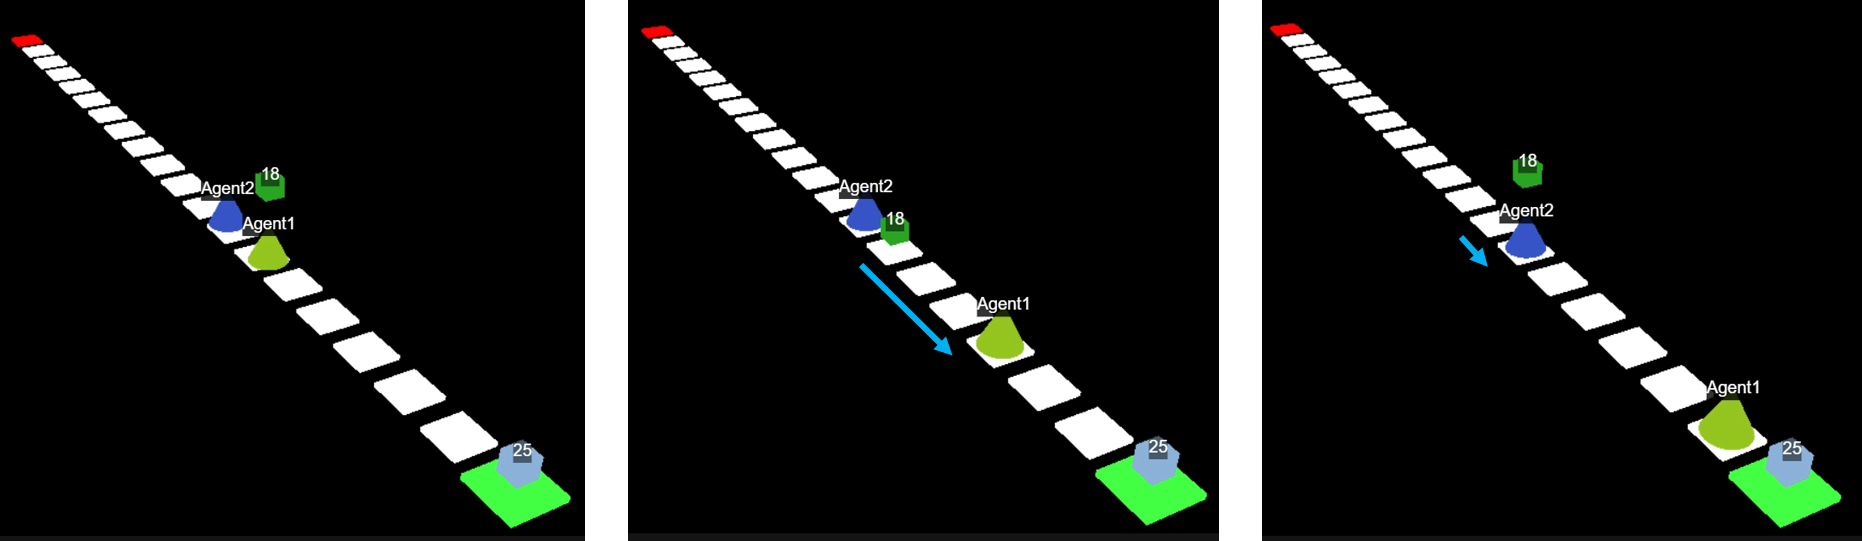
\includegraphics[width=\linewidth]{Images/exchange.png}
    \caption{Parcel exchange}
    \captionsetup{font=footnotesize}
    \caption*{The \textit{Agent1} detects its teammate, drops the parcels and goes away. The \textit{Agent2} goes to pickup the dropped parcels and will then deliver them to the base}
    \label{fig:exchange}
\end{figure}

% Spiegare se rimane bloccato
Sometimes an agent gets stuck because it cannot move in any direction, because it is blocked by his teammate. If this happens, it tells the other agent to move (through shared memory); the other agent pushes an intention with highest priority and moves away a few tiles, so the first agent has space to move and exchange the parcels correctly.


\subsection{Results in the Challenge 2}



Althought we placed 8\textsuperscript{th} among 14 teams, we further refined our code introducing the following new features:

\begin{itemize}
  \item \textbf{Map Partitioning via k‐Means:}  
    On the first game loop, we now optionally split the map between agents using k‐means (configurable with \texttt{USE\_MAP\_DIVISION}, \texttt{MAX\_TRIES\_KMEANS}, etc.). This ensures that each agent is responsible for its own sector, reducing overlap and improving parcel coverage.

  \item \textbf{Dynamic Base Reallocation and Path Fallback:}  
    We added a resilient \texttt{getBasePath(target)} routine that:  
    \begin{itemize}
      \item Attempts to compute a path to the given base tile.
      \item After a configurable number of failed tries (\texttt{BASE\_TRIES}), temporarily removes the blocked base tile from the map, waits \texttt{BASE\_REMOVAL\_TIME}, then restores it.
      \item Recomputes the nearest available base via \texttt{mapStore.nearestBase(this.me)} and updates \texttt{currentNearestBase}.
      \item Retries pathfinding up to \texttt{BASE\_SWITCH\_MAX\_TRIES} before giving up.
    \end{itemize}
\end{itemize}




\section{PDDL}
After building the \texttt{single} and \texttt{multi-Agents} another agent was created to assert the capabilities of the \texttt{PDDL} domain.

The new agent is almost entirely made up of \texttt{PDDL} code, and run on an online solver. It implicitly uses the \texttt{BDI} architecture, still sensing the environment, updating its belief, generating the desires to pick up and deposit parcels and generating a plan.

\subsection{Problem}

The automatically generated \texttt{deliveroo\_problem.pddl} file encapsulates one concrete snapshot of the game world that the planner must reason about. It follows the canonical PDDL layout:

\begin{enumerate}
  \item \textbf{(:objects)} declares every logical object that currently exists:
    \begin{itemize}
      \item the single agent (e.g., \textit{agent\_42});
      \item one symbol per visible parcel (e.g., \textit{p\_17});
      \item one symbol per known base (e.g., \textit{base\_1\_9});
      \item every walkable map tile (e.g., \textit{t\_5\_4}).
    \end{itemize}

  \item \textbf{(:init)} lists the ground facts that are \emph{true right now}:
    \begin{itemize}
      \item \textit{(at agent\_42 t\_4\_4)} — the agent’s current position;
      \item \textit{(parcel-at p\_17 t\_5\_4)} — parcel~\#17 is waiting on tile~$(5,4)$;
      \item \textit{(base-at base\_1\_9 t\_1\_9)} — a base occupies tile~$(1,9)$;
      \item \textit{ (adjacent t\_0\_2 t\_1\_2))} facts describing local connectivity.
    \end{itemize}

  \item \textbf{(\texttt{:goal})} a conjunctive goal that requires every currently known parcel to be delivered.

\end{enumerate}

All problem files are stored in the \texttt{PDDL} folder and are produced on the fly by \texttt{pddlTemplates\.js}.

\subsection{Domain}

Unlike the problem file, the domain file is \textbf{static}: it describes the immutable physics and rules of the \textbf{Deliveroo world}.

\paragraph{Types}
We have defined the following types:  \texttt{agent}, \texttt{parcel}, \texttt{base}, and \texttt{tile}.

\paragraph{Predicates}
\begin{itemize}
  \item\textbf{(at ?a ?t)} agent \textbf{a} is located on tile \textbf{t}.
  \item\textbf{(parcel-at ?p ?t)} parcel \textbf{p} is lying on tile \textbf{t}.
  \item\textbf{(carrying ?a ?p)} agent \textbf{a} is currently holding parcel \textbf{p}.
  \item\textbf{(base-at ?b ?t)} base \textbf{b} occupies tile \textbf{t}.
  \item\textbf{(delivered ?p)} parcel \textbf{p} has been delivered and it is no longer in play.
  \item\textbf{(adjacent ?t1 ?t2)} tiles \textbf{t1} and \textbf{t2} share an edge (undirected).
\end{itemize}

\paragraph{Actions}
Below is the definition of the three  actions that we have defined
\begin{itemize}[leftmargin=*]
  \item \textbf{move( ?a, ?from, ?to )}
    \begin{itemize}[leftmargin=1.5em]
      \item \textbf{Preconditions:}
        \begin{itemize}
          \item (at ?a ?from)
          \item (adjacent ?from ?to)
        \end{itemize}
      \item \textbf{Effects:}
        \begin{itemize}
          \item delete (at ?a ?from)
          \item add    (at ?a ?to)
        \end{itemize}
      \item \textbf{Intuition:} The agent leaves the source tile and appears on the destination tile.
    \end{itemize}

  \item \textbf{pickup( ?a, ?p, ?t )}
    \begin{itemize}[leftmargin=1.5em]
      \item \textbf{Preconditions:}
        \begin{itemize}
          \item (at ?a ?t)
          \item (parcel-at ?p ?t)
        \end{itemize}
      \item \textbf{Effects:}
        \begin{itemize}
          \item delete (parcel-at ?p ?t)
          \item add    (carrying ?a ?p)
        \end{itemize}
      \item \textbf{Intuition:} The parcel is removed from the ground and held by the agent.
    \end{itemize}

  \item \textbf{deposit( ?a, ?p, ?b, ?t )}
    \begin{itemize}[leftmargin=1.5em]
      \item \textbf{Preconditions:}
        \begin{itemize}
          \item (at ?a ?t)
          \item (base-at ?b ?t)
          \item (carrying ?a ?p)
        \end{itemize}
      \item \textbf{Effects:}
        \begin{itemize}
          \item delete (carrying ?a ?p)
          \item add    (delivered ?p)
        \end{itemize}
      \item \textbf{Intuition:} The parcel is dropped and marked as delivered.
    \end{itemize}
\end{itemize}


\subsection{Limitations}
Relying on an external PDDL solver brings two main challenges: network and solver latency, and world drift caused by the evolving game state. In the following, we first describe these issues in detail and then introduce our DEAR (Detect → Execution failure → Abort → Replan) approach as a remedy

\subsubsection*{Core Challenges}

The system relies on an external, online PDDL solver accessed via asynchronous API calls. When we request a plan:

\begin{itemize}
\item \textbf{Network and solver latency:} we must wait for the remote solver to compute and return a plan.
\item \textbf{World drift:} during this waiting period, the game world continues to evolve (e.g., other agents may pick up parcels, tiles may become blocked), so the returned plan may refer to parcels or states that no longer exist.
\end{itemize}

\emph{Example:} at time \textit{$t_{0}$} the agent asks for a plan to pick up parcel \textit{p\_1} at \textit{tile (5,4)}. Due to latency, the solver’s plan arrives at \textit{$t_{2}$}, but in the meanwhile, parcel \textit{p\_1} has already been collected by another agent, invalidating the plan.

\subsubsection*{Solution: DEAR }

In our implementation, if the agent encounters an execution error,such as being unable to move because another agent now occupies the target tile (a situation not reflected in the previously generated plan), it immediately stops executing the current plan. Using the most recent world model stored in \texttt{MapStore}, \texttt{ParcelsStore}, and \texttt{AgentStore}, we then invoke \texttt{getPlan()} again to generate a new, up-to date plan.

This approach, which we call \emph{DEAR}: {\textbf{Detect} $\rightarrow$ \textbf{Execution failure} $\rightarrow$ \textbf{Abort} $\rightarrow$   \textbf{Replan} guarantees that the agent never proceeds on outdated assumptions, providing robustness at the cost of additional solver calls.


\section{Documentation}
\subsubsection*{Documentation Generation}

\paragraph{Using JSDoc}
For automatic generation of our API documentation, we use \textbf{JSDoc}, a documentation generator for JavaScript that parses specially formatted comments within the source code. JSDoc recognizes standard tags (e.g., \texttt{@param}, \texttt{@returns}, \texttt{@description}, etc.) and produces a set of navigable HTML pages, making it easy to explore functions, classes, and their parameters. By using JSDoc, each function and class in our codebase is documented in a clear, up-to-date manner, directly from the source comments, minimizing the risk of outdated documentation.

\paragraph{Online Access}
The generated documentation is also accessible online at: \url{https://bandomatteo.github.io/Deliveroo/}

\paragraph{Local Generation}
To generate the documentation locally, simply run:
\begin{verbatim}
npm run generate-docs
\end{verbatim}


\section{Version Control and Project Management}
\begin{itemize}
  \item \textbf{GitHub Repository:} All code is hosted at: \url{https://github.com/bandomatteo/Deliveroo}, with a \texttt{main} branch for stable releases and \texttt{dev} branch for ongoing development.
  \item \textbf{Pull Requests} Significant modifications are submitted via pull requests.
  \item \textbf{GitHub Issues:} We track bugs and feature requests through issues labeled \texttt{bug}, \texttt{enhancement}, and \texttt{documentation}, organizing milestones for each release.
  \item \textbf{GitHub Projects:} We employ a Kanban board with \texttt{To do}, \texttt{In progress}, and \texttt{Done} columns to plan and monitor tasks in an Agile workflow.
\end{itemize}

\section{Future Works}
Building on our DEAR framework, we can further enhance the system’s robustness, performance, and scalability:

\paragraph{Hybrid approach}
    Use the PDDL solver only for a small part of the code, using more plain javascript and enabling to have more control over the agent.
    In this way the agent can be more complicated without changing much of the domain representation.

\paragraph{Embed a local PDDL solver} 
    Replace the remote API calls with an embedded planner running in-process.  
    This removes network-induced delays and world-drift inconsistencies, guarantees data coherence, and enables tighter integration between the planner and the world model.

\vspace{0.7cm}
We think that  adopting this change will dramatically reduce latency, eradicate API-related synchronization errors, and lay the foundation for a more resilient, high-throughput multi-agent planning platform.


%---------------------------------------------------------------------------
%  BIBLIOGRAPHY
%---------------------------------------------------------------------------
% Remember to insert here only the essential bibliography of your work
% \bibliography{bibliography.bib} % automatically inserted and ordered with this command 
% \printbibliography

\end{document}